\chapter{Current UCN Facility at TRIUMF}

% Based on simulations, a 40~$\mu$A of current produces a background of
% XXX mSev.

The current vertical UCN cryostat at TRIUMF is the same UCN cryostat
developed and tested at RCNP, Japan between 19xx and
2012(?)~\cite{masuda2002spallation,masuda2012spallation}.  In 2016,
the cryostat was shipped to triumf for further UCN experiments. These
experiments were essential for better understanding of the cryostat
and design of the next generation UCN source.  The vertical source was
modified to fulfill the safety requirements at TRIUMF (find where and
what those are.)  The current location of the vertical source is at
the meson hall experimental area.  A picture of the UCN facitity is
shown below.

The unique feature of the UCN source at TRIUMF is the combination of
spallation neutrons and superfluid helium for UCN production. This
will be discussed in detail in the following sections.
%%%%%%%%%%%%%%%%%%%%%%%%%%%%%

%%%%%%%%%%%%%%%%%%%%%%%%%%%%%
\section{UCN beamline}
%TRIUMF's proton beam is provided by a 520~Mev cyclotron.
TRIUMF produces negatively charged hydrogen ions from an ion
source. These ions are then accelerated in the 520~Mev cyclotron in an
outward spiral trajectory. A thin graphite stripper foil removes the
electrons from the hydrogen ion while protons can pass through. The
proton, because it is a positively charged particle, is deflected in
the outward direction due to the magnetic field and is directed to a
proton beam line. TRIUMF has four independent extraction probes with
various sizes of foils to provide protons simultaneously to up to four
beam lines.


The 120~$\mu$A beam (BL1A) enters the Meson Hall where the UCN
facility is located. The vertical UCN source was designed for a
maximum of 40~$\mu$A beam on target. As a result, only one third of
the beam can go to the UCN experimental area and the rest is shared
with different experimental facilities.

The microstructure of BL1A is in pulses with approximately 1~ms
periods of beam followed by a 50-100~$\mu$s periods of no beam.  This
is shown in Fig.~(\ref{fig:bl1u})~\cite{Nick_thesis}. A
kicker magnet kicks away 1/3 of the beam to BL1U. For most of the UCN
data taking, the beam was on for 1~min and off for 4~min. These times
are adjustable.

After the kicker magnet, the septum magnet bends the beam to the
target and the quadropoles focus the beam to the target.


\begin{figure}[h]
  \centering
  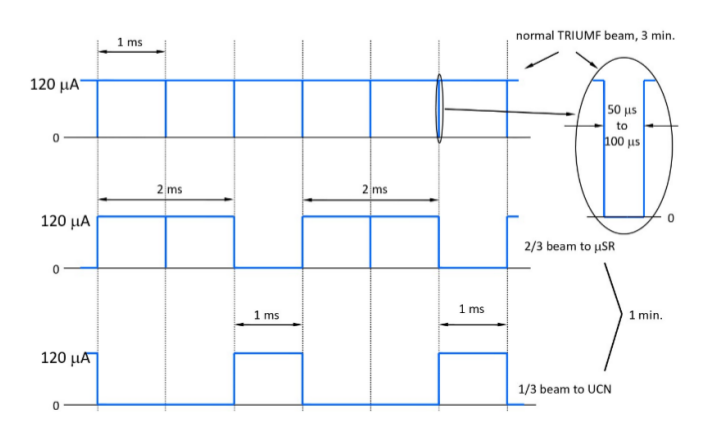
\includegraphics[width=0.9\textwidth]{bl1u.png}
  \caption{UCN beam structure. The top graph shows the 120~$\mu$A BL1A
    in 1~ms period of beam followed by a 50-100~$\mu$s of no
    beam. The middle graph shows the same beamline when the kicker
    magnet is on. The bottom graph shows the 1/3 of the beam that goes
    to the UCN area.}
  \label{fig:bl1u}
\end{figure}

\section{Radiation Sheilding}

%%%%%%%%%%%%%%%%%%%%%%%%%%%%%%%%%%%%%%%%%%%%%%%%%%%
%%% JUST TALKING ABOUT THE SETUP
%%%%%%%%%%%%%%%%%%%%%%%%%%%%%%%%%%%%%%%%%%%%%%%%%%%
\section{Vertical UCN Source at TRIUMF\label{sec:vertical_source}}


\subsection{D$_2$O Moderator}

\subsection{Helium Circulation}

\subsubsection{4 Kelvin Reservoir}

\subsubsection{1 Kelvin Pot}

\subsubsection{$^3$He Pot}

\subsubsection{Isopure Helium}


\section{Stages of UCN Production In The Source}
At TRIUMF, UCN is produced in three stages: Spallation, moderation and
conversion. Fig.~(\ref{fig:ucn_production_stages}) shows a schematic of
this process.

\begin{figure}[h]
  \centering
  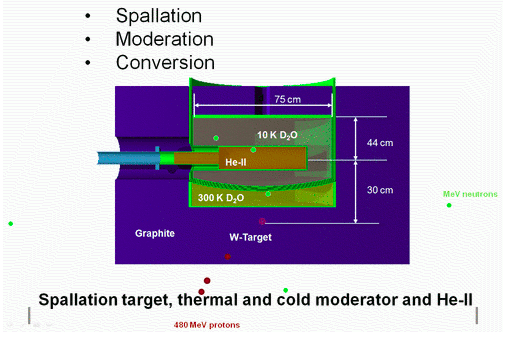
\includegraphics[width=0.9\textwidth]{ucn_production_stages.png}
  \caption{blah}
  \label{fig:ucn_production_stages}
\end{figure}
%\subsection{Neutron Spallation Target}

The neutrons are produced through the spallation process by hitting a
Tungsten target by the proton beam. Spallation is refered to a nuclear
reaction where high energy particles interact with atomic
nucleus. This process creates many high energy neutrons and background
radiation.  The target is surrounded by several blocks of lead and
graphite. These fast neutrons
are reflected and moderated down and enter the warm D$_2$O moderator at room temperature~(300 K) and become thermal
neutrons with an energy of 0.025~eV and the speed of 2.2~km/s.

%\subsection{Neutron Moderation}
Iced heavy water at 20~K is used as a cold moderator. After passing
through the warm D$_2$O, thermal neutrons enter the the cold moderator
and become cold neutrons. These neutrons have the speed of several
hundreds of meter per second.

%\subsection{Neutron Conversion}
The last stage is when the slow neutrons enter the isotopically pure superfluid helium
at 0.84 to 0.92~K. UCN is produced as a result of phonon transitions
inside the superfluid helium as discussed in section~\ref{sec:ucn_with_heII}.


\section{D$_2$O Solidification}
The D$_2$O vessel has a capacity of 100~L. At first, 14~L of liquid
D$_2$O gets injected to the vessel. This is followed by adding 11~L of
D$_2$O to the vessel over 8 times.  After filling up the vessel,
Gifford McMahon refrigerators solidify the heavy water and further
cool it down to 10~K. The process of icing the heavy water takes about
6 days and cooling it down takes another XXX days.

\section{Data Acquisition System\ref{sec:DAQ}}
Here talk about the EPICS and PLC and put pictures. I can also use
stuff from student's reports.

\section{UCN Detectors}
Talk about how each detector works.
\subsection{$^6$Li Detector\label{sec:Li6detector}}
The main detector used during the UCN measurements~(See
Chapter~\ref{chap:UCNresult}) is a $^6\mathrm{Li}$ glass based scintillator
detector designed and built at the University of Winnipeg for the
TUCAN nEDM experiment at
TRIUMF~\cite{jamieson2017characterization}. Since $^6\mathrm{Li}$ has a high
neutron capture cross-section~(order of $10^5$ bn) at UCN energies,
the scintillator glass is doped with it. The charged particles in the
reaction
\begin{equation}
^6Li + n \rightarrow \alpha (2.05~\mathrm{MeV}) + t (2.73~\mathrm{MeV})
\end{equation}
are detected. To reduce the effect of $\alpha$ or triton escaping the
glass, a layer of 60~$\mu$m thick depleted $^6\mathrm{Li}$ glass (GS30), on top
of a layer of 120~$\mu$m thick dopped $^6\mathrm{Li}$ (GS20) were optically
bonded. This design allows the resultant particles to deposit all of
their energy within the scintillating
glass. Table~\ref{tab:scintillator} shows the content and density of
those $^6\mathrm{Li}$ scintillators.

\begin{table}[h!]
  \centering
  \label{tab:scintillator}
  \begin{tabular}{|c|c|c|}
    \hline
    Scintillator & GS20~($^6\mathrm{Li}$ Enriched) & GS30~( $^6\mathrm{Li}$ depleted) \\
    \hline
    Total Li content (\%) & 6.6 & 6.6 \\
    \hline
    $^6\mathrm{Li}$ fraction (\%) & 95 & 0.01 \\
    \hline
    $^6\mathrm{Li}$ desity~(cm$^{-3}$) & $1.716 \times 10^{22}$ & $1.806 \times 10^{18}$ \\
    \hline
  \end{tabular}
  \caption{Properties of the glass scintillators}
\end{table}


Making the scintillating Li glass as thin as possible reduces the
sensitivity to $\gamma$-ray scintillating backgrounds and and thermal
neutron captures. The mean range of the $\alpha$ is 5.3~$\mu$m and the
mean range of the triton is 34.7~$\mu$m. This means that if the
thickness of the scintillator is less than 50~$\mu$m, the resultant
particles escape before stopping which gives rise to an efficiency
loss.  In order to handle high UCN rates of up to \~1~MHz, the
$^6\mathrm{Li}$ detector face is segmented into 9 tiles~(See
Fig.~\ref{fig:Li6detector}). The scintillation light is then guided
through ultra-violet transmitting acrylic light-guide to its
corresponding Photomultiplier Tube~(PMT) outside the vaccum region of
the detector.

\begin{figure}[h]
  \centering
  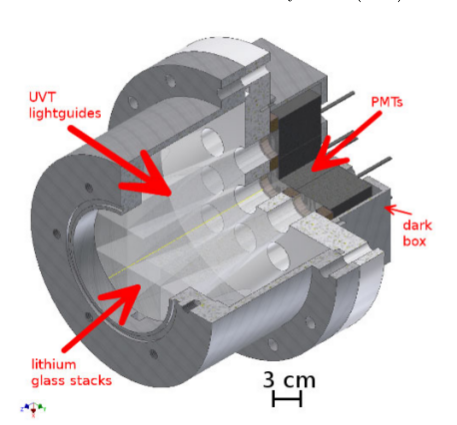
\includegraphics[width=0.5\textwidth]{Li6detector.png}
  \caption{3D drawing of the $^6$Li detector and its enclosure. The
    enclosure is made of Al, and the rim of the adapter flange which
    UCN can hit is ccoated with 1~$\mu$m Ni by thermal evaporation. }
  \label{fig:Li6detector}
\end{figure}

The data acquisition with this detector includes a CAEN V1720
digitizer which has a Pulse-Shape Discrimination~(PSD) firmware that
triggers on pulses below a certain threshold for each channel. Every
4~ns the digitizer samples the waveform which is then digitized to a
voltage on a 2~V scale into an ADC value between 0 and 4096. Each
channel of the digitizer sends a trigger whenever the number of counts
in the ADC goes below a certain baseline~(pedestal) value. The PSD
calculates the sum of the signal below the baseline for two time
windows: $t_s = 40$~ns (short gate) and $t_L = 200$~ns~(long
gate). The short gate is chosen in a way to contain all of the charge
for the $\gamma$-ray interactions in the light-guide. The ADC sum for
during the long gate below the baseline is calle $Q_L$~(read charge
long) and for during the short gate below the baseline is called
$Q_S$. Charge long has the total charge deposti for the neutron
capture events. The PSD value is defined as
\begin{equation}
  \label{eq:psd}
  \mathrm{PSD} = \frac{\left( Q_L - Q_S\right)}{Q_L}
\end{equation}  
which is the amount of charge in the tail of an event.

Jamieson {\it{et al.}} showed that the absolute efficiency of this
detector is $89.7^{+1.3}_{-1.9}$~\% with a background contamination of
$0.3 \pm 0.1$~\%~\cite{jamieson2017characterization}. The detector is
stable at the 0.06~\% level or better, and that the variation in the
efficiency between the detector tiles is less than 5~\%.
\subsection{$^3$He Detector}




%\begin{description}
%\item{An intro to whatever goes into this chapter}

%\item{Start by showing a nice drawing and then talk about each
 % componet of the facility:}
  
%\item{about proton beam that we get, the magnets and basically how the
%  beam reaches the target and how it looks like (Where can I get this
%  information? Is it written somewhere?)}
  
%\item{A short introduction to say the stages of UCN production and why
%  we need the vertical cryostat (Link to the next stage)}
  
%\item{It also has to be mention that it is the same vertical sourcse
%  as was used at the RCNP and some modifications were made to meet the
%  requirements at triumf. (Where can I find what modifications were
%  made?) Agian this has to be just as a link to the next chapter(maybe?)}
  
%\item{The target and shielding (with pictures?), only a few
%  paragraphs}
  
%\item{Moderation: D2O system (I can use Ryohei's thesis I guess)}
  
%\item{conversion. There is a whole chapter dedicated to the UCN
%  cryogenics. I have to go through details (not too much) of how the
%  cryostat works. I can borrow some infromation from Ryohei's
%  thesis. I am not sure how much of it is related to the next
%  chapter.}
 

%\item{Data acquisition system, epics and plc, I guess there are useful
%  informaion in Sean Vanbergen's report that I can use for this
%  section}
  
%\item{what else?}

%\end{description}
